\section{Methodology}\label{sec:meth}
\vspace{-1mm}
This section outlines the methodology used for evaluating the mathematical reasoning capabilities of the selected LLMs. Our approach prioritized accuracy, fairness, and transparency throughout each step, involving careful preparation and grading procedures.

\begin{figure*}[t]
    \centering
    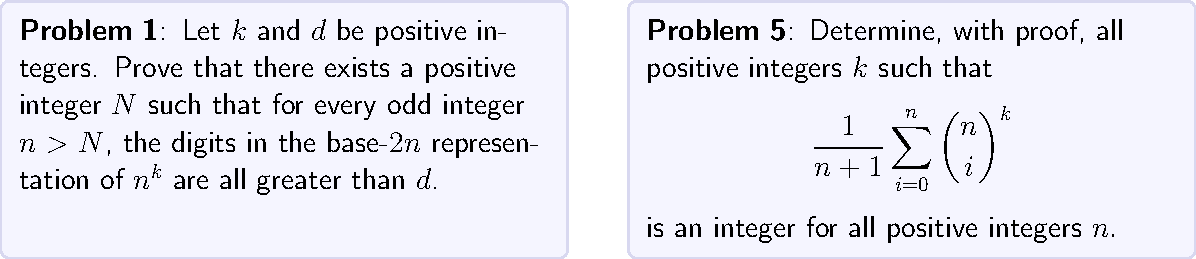
\includegraphics[width=0.95\linewidth]{figures/figure_1.pdf}
    \vspace{-2mm}
    \caption{Two problems of USAMO 2025. The other problems are available in \cref{app:problems}}
    \label{fig:problems}
    \vspace{-0.2in}
\end{figure*}
\vspace{-2mm}

\subsection{Problem Selection and Preparation}
\vspace{-2mm}
We selected the USAMO 2025, a highly prestigious mathematics competition comprising six proof-based problems administered over two days, as our benchmark. This competition aligns perfectly with our evaluation objectives, as the questions are challenging, require detailed proofs for full credit, and are uncontaminated. In \cref{fig:problems}, we present two problems from the competition, with the remaining four available in \cref{app:problems}.

For evaluation, we provided each model with the problems, prompting them explicitly to produce comprehensive and detailed proofs formatted in \LaTeX. The full prompt instructions and details of used hyperparameters are available in \cref{app:exp_prompt}. To reduce variance, each model solved every problem four separate times. Solutions, excluding thought traces, were anonymized and converted into PDF format for grading. Both \grok{} and \geminipro{} were evaluated after our initial grading and were therefore not fully anonymous when presented to the judges.
\vspace{-2mm}

\subsection{Judge Selection and Training}
\vspace{-1mm}
Our grading team consisted of four experts, each having substantial mathematical problem-solving experience as former national IMO team members or having participated in final-stage team selection processes for their countries. Prior to the grading, judges received instructions detailing evaluation goals and methodologies. These guidelines are accessible in our GitHub repository. A trial run with three USAMO 2024 problems was conducted to familiarize evaluators with the grading approach and resolve ambiguities. Small misunderstandings were clarified during this session.

\subsection{Grading Procedure}

Each of the six problems from USAMO 2025 was independently evaluated by two evaluators, with each judge responsible for grading three unique problems. This double grading method, modeled after the IMO's evaluation process, ensures consistency in our grading and decreases personal biases.

Since the official USAMO does not release standard solutions or grading schemes, we carefully developed a standardized grading scheme for each problem, drawing from reliable mathematical community resources, particularly the Art of Problem Solving (AoPS) forums. All solutions from these sources were verified by our evaluators for accuracy before creating the grading scheme. Following USAMO conventions, each solution was graded out of a maximum of seven points with partial credit given for significant and meaningful progress. The finalized grading schemes are available in our GitHub repository and displayed on our website. An example can be found in \cref{app:exp_grading}.

Judges independently reviewed each assigned solution against the pre-established grading scheme. When a solution did not perfectly align with the scheme, the approach was awarded points where appropriate. Each judge documented their reasoning, including justification for each partial credit awarded. These notes are also accessible on our website, with an example provided in \cref{app:exp_grading}.

Evaluators also documented prominent failure modes observed during grading. A "failure mode" was defined as the first instance of incorrect or inadequately explained reasoning, such as flawed logic, unjustified assumptions, mathematical inaccuracies, or computational mistakes. Specifically, mistakes were categorized into four classes:

\vspace{-2mm}
\begin{itemize}[leftmargin=25pt]
\setlength\itemsep{0.01em}
\item \textbf{Logic:} Errors due to logical fallacies or unjustified leaps disrupting the reasoning.
\item \textbf{Assumption:} Errors coming from the introduction of unproven or incorrect assumptions that undermined subsequent steps.
\item \textbf{Creativity:} Errors resulting from fundamentally incorrect solution strategies due to the inability to identify the correct approach.
\item \textbf{Algebra/Arithmetic:} Errors arising from critical algebraic or arithmetic miscalculations.
\end{itemize}

We show examples of these errors in \cref{app:error_mode_examples}.

Additionally, noteworthy behaviors or trends in model-generated solutions were systematically logged for further analysis. These observations were used to identify common pitfalls and areas for improvement in the models' reasoning capabilities and are presented in \cref{sec:discussion}.